\documentclass[10pt,a4paper]{article}
\usepackage[utf8]{inputenc}
\usepackage[italian]{babel}
\usepackage{amsmath}
\usepackage{amsfonts}
\usepackage{amssymb}
\usepackage{graphicx}
\usepackage{siunitx}
\usepackage[left=2cm,right=2cm,top=2cm,bottom=2cm]{geometry}
\newcommand{\rem}[1]{[\emph{#1}]}
\newcommand{\exn}{\phantom{xxx}}
\usepackage[italian]{babel}
\usepackage[utf8]{inputenc}
\usepackage{siunitx}
\usepackage{graphicx}
\usepackage{xcolor}
\usepackage{amsfonts}
\usepackage{amsmath}
\usepackage{amsthm}
\usepackage{tikz}
\usepackage{pgfplots}
\usepackage{enumitem}
\usepackage{siunitx}
\date{\today}
\usetikzlibrary{shapes.geometric,calc,matrix,arrows,snakes,shapes,patterns}
\title{Esercitazione 10B: Caratteristiche porte logiche e semplici circuiti logici}
\author{Massimo Bilancioni, Alessandro Foligno}
\begin{document}	
\maketitle
	
	\section{Caratteristiche statiche}
	Si monta il circuito come in figura,, utilizzando i resistenze con valori nominali:\[R_2=100\Omega \]
	$R_1\approx2080(scala 20k)\Omega$ ha un ingresso variabile che permettere di utilizzarla come partitore variabile di tensione (e quindi di mettere l'ingresso ad H/L).
	Per misurare VIL, VOH vario il potenziometro finchè non vedo il valore in uscita variare bruscamente. Analogamente con VIH, VOL (solo che abbasso la tensione in ingresso finchè non osservo variazioni brusche).
	\\Ottengo, come stima:
	\begin{enumerate}
		\item $V_{IL}\approx0.9 V,~V_{IL~nominale}=$
		\item $V_{IH}		\approx 1.5V,~V_{IH~nominale}=$
		\item $V_{OL}\approx0.1V,~V_{OL~nominale}=$
		\item $V_{OH}\approx5V,~V_{OH~nominale}=$
	\end{enumerate}
	Successivamente si è tracciato un grafico $V_{in}/V_{out}$ con i dati riportati nella seguente tabella:
	\section{Caratteristiche dinamiche}
\textcolor{red}{correggere in base all'immagine l'ampiezza dell'onda quadra, aggiungere erroe ai tempi, confronto finale può essere colpa del generatore che non è abbastanza veloce a cambiare}
Abbiamo inviato un'onda quadra con valori  $0-5 \si{\volt}$ in ingresso. Nelle figure compaiono l'ingresso (arancio) e l'uscita (blu) rispettivamente negli istanti in cui l'ingresso passa da basso ad alto e da alto a basso.
Nel primo caso misuriamo $t_{PHL}= 20 \si{\nano\second}$ nel secondo  misuriamo $t_{PLH} = 40\si{\nano \second}$.
Nel datasheet sono riportati i valori tipici: $t_{PHL}= 10 \si{\nano\second}$, $t_{PLH} = 9\si{\nano \second}$ e quello massimo $t_{PHL}^{MAX}= t_{PLH}^{MAX}= 15 \si{\nano\second}$.


\section{Costruzione di circuiti logici elementari}
Si è verificato il comportamento della porta NAND tramite i led con il circuito mostrato in \textcolor{red}{figura}.

Il circuito AND è stato costruito con due porte NAND secondo lo schema mostrato in Figura (\ref{fig:and}).

\begin{figure}
			\centering
			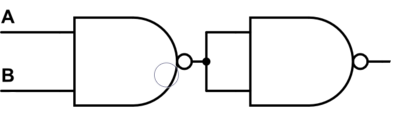
\includegraphics[scale=0.60]{and}
			\caption{schema porta AND}
			\label{fig:and}
\end{figure}
Per il circuito OR  si sono usate tre porte NAND, Figura (\ref{fig:or}).
\begin{figure}
			\centering
			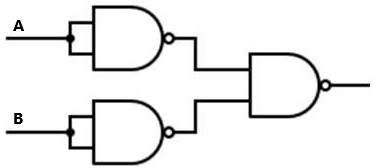
\includegraphics[scale=0.85]{or}
			\caption{schema porta OR}
			\label{fig:or}
\end{figure}
Il circuito XOR  è stato realizzato con quattro porte NAND, Figura (\ref{fig:xor}).
\begin{figure}
			\centering
			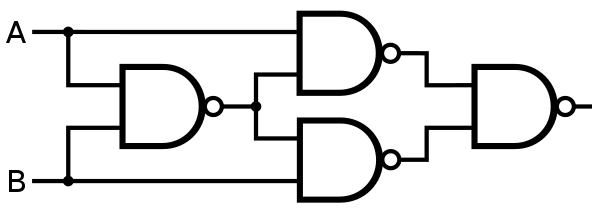
\includegraphics[scale=0.55]{xor}
			\caption{schema porta XOR}
			\label{fig:xor}
\end{figure}
Il sommatore a due bit è stato costruito con cinque porte NAND: una in meno rispetto alla somma AND $+$  XOR perchè una porta era in comune, Figura (\ref{fig:som}).
\begin{figure}
			\centering
			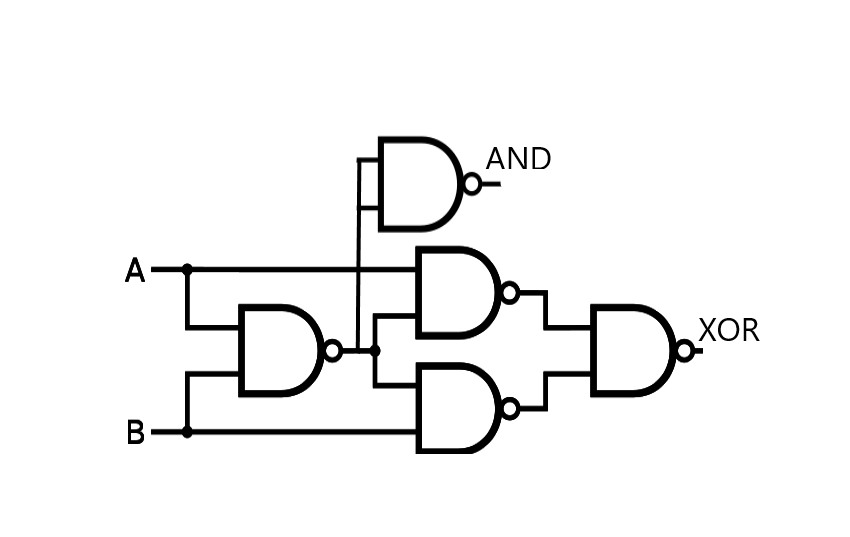
\includegraphics[scale=0.55]{sommatore}
			\caption{schema sommatore a due bit}
			\label{fig:som}
\end{figure}
\end{document}